\chapter{Introduction}

This project explores a novel matrix-based technique for calculating the upper bound of instruction level parallelism
in a program. This project shows that this approach offers better performance than traditional analysis techniques,
at the cost of greater use of memory.

\section{Background: ILP and limit studies} \label{intro:background}

\textit{Instruction level parallelism} (ILP) is the simultaneous execution of independent instructions in a computer processor~\cite{hennessy_patterson}.
A pair of instructions from a thread of execution are independent when there exist no dependencies (specifically data,
control or structural dependencies) between them. An instruction dependent on a previous one must be executed strictly
after the former has completed execution to ensure correct execution of the entire program.

Modern superscalar processors exploit ILP to increase throughput and hide latency \cite{shen2013modern}. The absolute limit of 
exploitable ILP is dependent on the structure of the executed program. A dynamic execution of a program will have a
`critical path' of instructions, each data-dependent on the previous, that have to be executed sequentially.

To understand these theoretical limits, studies are conducted to measure the maximum ILP available, through analysis 
on dynamic execution traces. Tools are used to build a \textit{dynamic dependency graph} (DDG), where nodes represent dynamically 
executed instructions, and edges represent the dependencies between them. The program's maximum available ILP is 
calculated by dividing the total number of executed instructions by the length of the longest path (the critical path)
through the DDG \cite{wall-ilp}. An example DDG is shown in Figure \ref{fig:DDG}.

\begin{figure}[ht]
    \rule{\textwidth}{0.5pt}\vspace{0.2cm}

    \centering
    % LEFT SIDE: Execution Trace
    \begin{minipage}[t]{0.35\textwidth}
        \centering
        \textit{Execution Trace} \\[1em]
        {\ttfamily\small
        \begin{tabular}{l}
        load r0, A \\
        load r1, B \\
        r4 $\leftarrow$ r0 + r1 \\
        load r2, C \\
        load r3, D \\
        r5 $\leftarrow$ r2 + r3 \\
        r6 $\leftarrow$ r4 + r5 \\
        store r6, S
        \end{tabular}}
    \end{minipage}
    \hfill
    % RIGHT SIDE: Dynamic Dependency Graph
    \begin{minipage}[t]{0.55\textwidth}
        \centering
        \textit{Dynamic Dependency Graph} \\[1em]
        \begin{tikzpicture}[scale=0.8, every node/.style={transform shape}]
            \node (a0) {load r0, A};
            \node [right=0.5cm of a0] (a1) {load r1, B};
            \node [right=0.5cm of a1] (a2) {load r2, C};
            \node [right=0.5cm of a2] (a3) {load r3, D};

            \node (b0) [below=1cm of $(a0.south)!0.5!(a1.south)$] {r4$\leftarrow$r0+r1};
            \node (b1) [below=1cm of $(a2.south)!0.5!(a3.south)$] {r5$\leftarrow$r2+r3};

            \node (c0) [below=1cm of $(b0.south)!0.5!(b1.south)$] {r6$\leftarrow$r4+r5};
            \node (d0) [below=0.8cm of c0] {store r6, S};

            \draw[->] (a0) -- (b0);
            \draw[->] (a1) -- (b0);
            \draw[->] (a2) -- (b1);
            \draw[->] (a3) -- (b1);
            \draw[->] (b0) -- (c0);
            \draw[->] (b1) -- (c0);
            \draw[->] (c0) -- (d0);
        \end{tikzpicture}
    \end{minipage}

    \caption{Example dynamic dependency graph \cite{ddg}}
    \label{fig:DDG}
    \vspace{0.1cm}\rule{\textwidth}{0.5pt}
\end{figure}

\section{Motivation} \label{intro:motivation}

Traditionally, limit studies compute this longest path using a single-pass sequential sweep over the execution trace.~\cite{wall-ilp, ilp-spec95, perpi}
At each step they calculate the length of dependency paths ending at each register, and pick out the longest path at the 
end of the trace. Because the algorithm traverses the trace sequentially to propagate
dependencies, it cannot be heavily parallelised, nor can it exploit the memoisation of program stuctures such as loops.
This sequentiality limits the ability to handle realistic execution traces containing trillions of instructions,
which is important for capturing the effects of long-term dependencies found in complex, real-world 
software. Furthermore, this analysis is rarely a single-pass operation. Limit studies evaluate programs across comprehensive 
benchmark suites under various parameters, such as restricted instruction windows or different branch prediction models~\cite{wall-ilp, future-ilp, ilp-spec95}.

To break this sequential bottleneck, Chadwick \cite{Chadderz} proposes a matrix-based approach. By representing instruction 
dependencies as matrices, and using matrix multiplication in the max-tropical semiring, computing the longest path in
the DDG becomes a problem of reducing a large expression of matrix multiplications.
Because matrix multiplication is associative, the expression can be evaluated in any order, and intermediate results 
fully encode the dependency information of the instructions they range over. This enables a range of optimisations when 
computing ILP limits, including thread-parallelisation of computations and memoisation of repetitive intermediate results.
One additional benefit of the associativity of the matrix expression is that it trivialises instruction window scaling.
Consider three windows of instructions: A, B, and C (which is comprised of windows A and B consecutively).

% \begin{center}
% 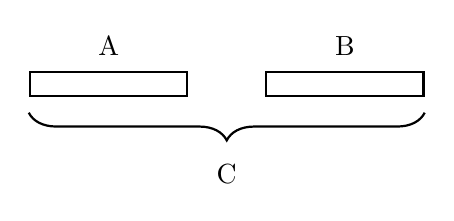
\begin{tikzpicture}

    % Define the two rectangles
    \node[draw, rectangle, minimum width=2cm, minimum height=0.3cm, thick] (boxA) at (0,0) {};
    \node[draw, rectangle, minimum width=2cm, minimum height=0.3cm, thick] (boxB) at (3,0) {};

    % Add labels A and B above the rectangles
    \node at (boxA.north) [above=2pt] {A};
    \node at (boxB.north) [above=2pt] {B};

    % Draw the brace spanning from the bottom-left of A to the bottom-right of B
    % 'mirror' puts the brace below the line
    \draw [decorate, decoration={brace, amplitude=10pt, mirror}, thick] 
        ([yshift=-0.2cm]boxA.south west) -- ([yshift=-0.2cm]boxB.south east) 
        node[midway, below=15pt] {C};

\end{tikzpicture}

% \end{center}

To compute ILP information for each window, the traditional approach must be executed 3 times, once for 
each window. However, the matrix-based approach will only need to run twice, on A and B, and the dependency 
information matrix for C can simply be obtained by multiplying the result matrices from A and B.

\section{Contributions}

In this project, I explore several approaches for offline computation of the upper limit of ILP in a program, and
compare their performance.
The first is a sequential approach mirroring the classical trace-analysis techniques, based on the PerPI tool \cite{perpi}. We will 
refer to this as the `naive baseline' throughout the project.
I then explore Chadwick's matrix-based approach, implementing a series of algorithmic and hardware-level optimisations.
Specifically, I use sparse matrix representations to reduce memory overhead, and develop data-level heuristics to 
determine optimal expression evaluation orders. Finally, I introduce parallel optimisations, leveraging multi-threading 
and accelerator-level parallelism to distribute the computational workload.

I show experimentally in Section \ref{eval:holistic-pipeline}
that a single-threaded pipeline equipped with the data-driven optimisations matches or beats the performance 
of the naive baseline. Furthermore, by distributing expression reduction and matrix multiplication workloads over 
multiple cores, I show that the parallel approach is at least twice as fast as the baseline,
demonstrating the scalability of the matrix-based approach in analysing large execution traces.
